\documentclass[border=1cm]{standalone}

\usepackage{tikz}

\usetikzlibrary{calc, angles}
\begin{document}
    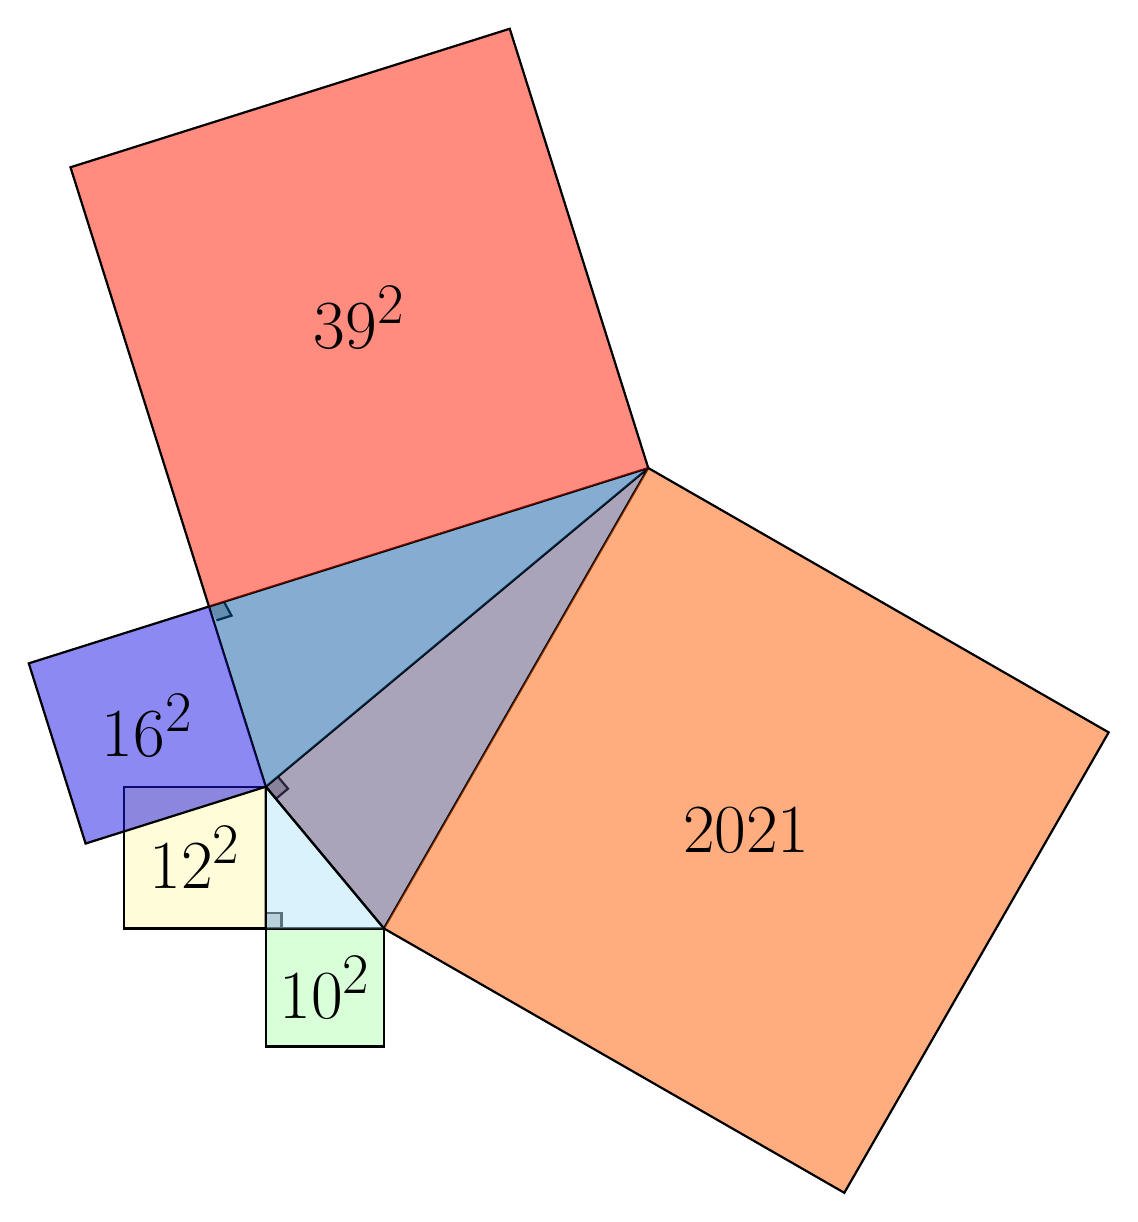
\begin{tikzpicture}[thick, scale=0.15]
        \coordinate (o) at (0,0);
        \coordinate (a) at (-10,12);
        \coordinate (k) at (-22,0);
        \coordinate (l) at (-10,-10);
        \coordinate (m) at (-10,0);
        \coordinate (c) at ($ (a)!42.1545cm!90:(o) $);
        \coordinate (d) at ($ (o)!44.9555cm!-90:(c) $);
        \coordinate (e) at ($ (c)!44.9555cm!90:(o) $);
        \coordinate (f) at ($ (c)!39cm!-22.3062:(a) $);
        \coordinate (g) at ($ (f)!16cm!-90:(a) $);
        \coordinate (h) at ($ (a)!16cm!90:(f) $);
        \coordinate (i) at ($ (f)!39cm!90:(c) $);
        \coordinate (j) at ($ (c)!39cm!-90:(f) $);
        \draw pic [draw, fill=gray!50, angle radius=2mm] {right angle = o--m--a};
        \draw pic [draw, fill=gray!50, angle radius=2mm] {right angle = o--a--c};
        \draw pic [draw, fill=gray!50, angle radius=2mm] {right angle = o--f--c};
        \draw[fill=yellow!30, fill opacity=0.5] (k) rectangle(a);
        \draw[fill=green!30, fill opacity=0.5] (l) rectangle(o);
        \draw[fill=olive!30!blue, fill opacity=0.5] (o)--(a)--(c) (o)--(c);
        \draw[fill=red!30!orange, fill opacity=0.5] (o)--(d)--(e)--(c);
        \draw[fill=gray!20!green!40!blue, fill opacity=0.5] (c)--(f)--(a);
        \draw[fill=orange!50!yellow!10!blue, fill opacity=0.5] (a)--(h)--(g)--(f);
        \draw[fill=red!80!orange, fill opacity=0.5] (f)--(i)--(j)--(c);
        \draw[fill=cyan!30, fill opacity=0.5] (o)--(a)--(m);
        \Huge
        \node at ($0.5*(o)+0.5*(l)$) {$10^2$};
        \node at ($0.5*(k)+0.5*(a)$) {$12^2$};
        \node at ($0.5*(o)+0.5*(e)$) {$2021$};
        \node at ($0.5*(h)+0.5*(f)$) {$16^2$};
        \node at ($0.5*(f)+0.5*(j)$) {$39^2$};
    \end{tikzpicture}
\end{document}